\section{Resultados y discusión}
\label{sec:resultados}

Esta sección presenta los resultados de las mediciones descritas en la
Sección~\ref{sec:metodologia}. Se exponen primero los costos de cada etapa, después el costo de
obtener la primera prueba y su amortización a lo largo de varias pruebas y luego el costo de
verificar las pruebas en la cadena de destino. Finalmente, se discuten los resultados en relación
con el diseño del puente y con la pregunta de investigación.

\subsection{Costo por etapa}
\label{sec:resultados_etapas}

La Tabla~\ref{tab:resultados_etapas} reúne el tiempo de reloj, la memoria residente máxima y el
uso del procesador de cada etapa, y las Figuras~\ref{fig:resultados_tiempo}
y~\ref{fig:resultados_memoria} representan los dos primeros. Todas las etapas concluyeron con
código de salida cero. La ejecución del programa de SP1 informó 66\,378\,401 ciclos de la máquina
virtual y confirmó la validez de la firma agregada.

\begin{table}[htbp]
	\centering
	\caption{Tiempo, memoria residente máxima y uso del procesador por etapa en Noir y en SP1.}
	\label{tab:resultados_etapas}
	\small
	\setlength{\tabcolsep}{4pt}
	\begin{tabular}{>{\raggedright\arraybackslash}p{2.3cm} >{\raggedleft\arraybackslash}p{2.4cm} >{\raggedleft\arraybackslash}p{1.85cm} >{\raggedleft\arraybackslash}p{1.3cm} >{\raggedleft\arraybackslash}p{2.4cm} >{\raggedleft\arraybackslash}p{1.85cm} >{\raggedleft\arraybackslash}p{1.3cm}}
		\toprule
		& \multicolumn{3}{c}{\textbf{Noir}} & \multicolumn{3}{c}{\textbf{SP1}} \\
		\cmidrule(lr){2-4} \cmidrule(lr){5-7}
		\textbf{Etapa} & \textbf{Tiempo} & \textbf{Memoria} & \textbf{CPU} & \textbf{Tiempo} &
		\textbf{Memoria} & \textbf{CPU} \\
		\midrule
		Compilación & 1 h 28 min 17 s & 86,7 GiB & 63\,\% & 0,58 s & 0,12 GiB & 101\,\% \\
		\addlinespace
		Testigo o ejecución & 1 min 35,3 s & 4,4 GiB & 100\,\% & 36,7 s & 6,8 GiB & 975\,\% \\
		\addlinespace
		Clave de verificación & 59,5 s & 17,2 GiB & 412\,\% & 5,6 s & 0,58 GiB & 703\,\% \\
		\addlinespace
		Prueba & 1 min 24,4 s & 19,0 GiB & 763\,\% & 17 min 9,5 s & 86,4 GiB & 1147\,\% \\
		\addlinespace
		Verificación & 0,01 s & 8,6 MiB & 160\,\% & \multicolumn{3}{c}{Incluida en la etapa de
		prueba} \\
		\bottomrule
	\end{tabular}
\end{table}

\begin{figure}[htbp]
	\centering
	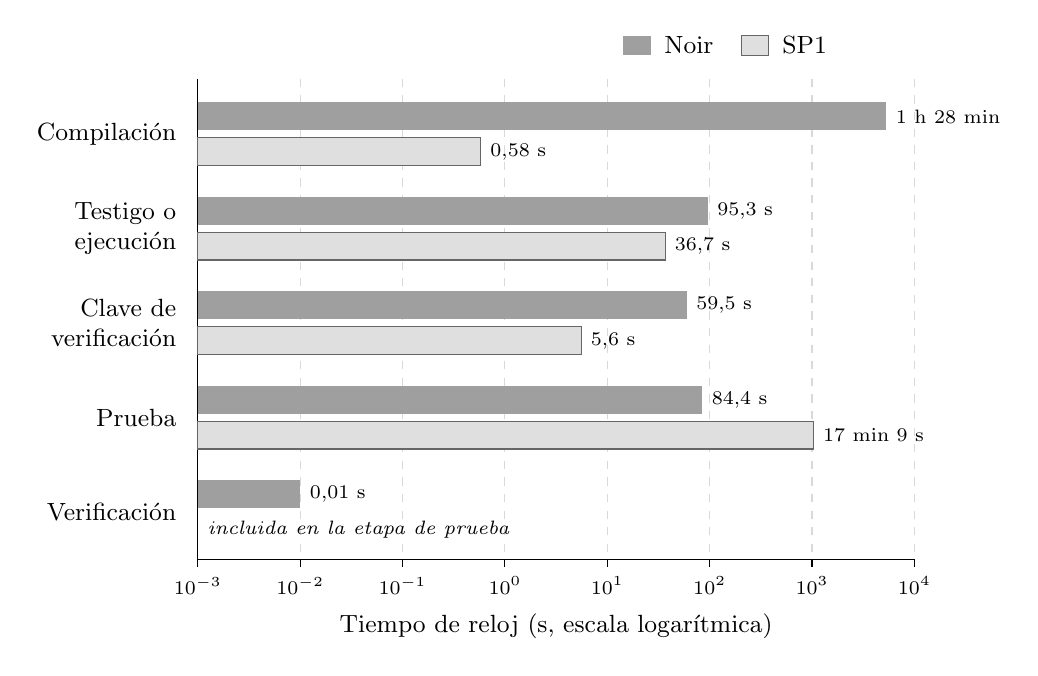
\begin{tikzpicture}[
		etapa/.style={anchor=east, font=\small, align=right},
		valor/.style={anchor=west, font=\scriptsize}
		]
		% Grilla y eje logarítmico: x = 1,3 (log10 t + 3)
		\foreach \i/\e in {0/-3, 1/-2, 2/-1, 3/0, 4/1, 5/2, 6/3, 7/4} {
			\draw[gray!30, dashed] (1.3*\i, 0.7) -- (1.3*\i, -5.4);
			\draw (1.3*\i, -5.4) -- (1.3*\i, -5.5) node[below, font=\scriptsize] {$10^{\e}$};
		}
		\draw (0, 0.7) -- (0, -5.4) -- (9.1, -5.4);
		\node[font=\small] at (4.55, -6.25) {Tiempo de reloj (s, escala logarítmica)};

		\foreach \y/\nombre/\ln/\vn/\ls/\vs in {
			0/Compilación/8.741/{1 h 28 min}/3.592/{0,58 s},
			-1.2/{Testigo o\\ejecución}/6.473/{95,3 s}/5.934/{36,7 s},
			-2.4/{Clave de\\verificación}/6.207/{59,5 s}/4.868/{5,6 s},
			-3.6/Prueba/6.404/{84,4 s}/7.816/{17 min 9 s}} {
			\node[etapa] at (-0.15, \y) {\nombre};
			\fill[gray!75] (0, \y+0.05) rectangle (\ln, \y+0.4);
			\node[valor] at (\ln, \y+0.225) {\vn};
			\fill[gray!25, draw=black!60] (0, \y-0.4) rectangle (\ls, \y-0.05);
			\node[valor] at (\ls, \y-0.225) {\vs};
		}
		\node[etapa] at (-0.15, -4.8) {Verificación};
		\fill[gray!75] (0, -4.75) rectangle (1.3, -4.4);
		\node[valor] at (1.3, -4.575) {0,01 s};
		\node[valor, font=\scriptsize\itshape] at (0, -5.025) {incluida en la etapa de prueba};

		% Leyenda
		\fill[gray!75] (5.4, 1.0) rectangle (5.75, 1.25);
		\node[valor, font=\small] at (5.8, 1.125) {Noir};
		\fill[gray!25, draw=black!60] (6.9, 1.0) rectangle (7.25, 1.25);
		\node[valor, font=\small] at (7.3, 1.125) {SP1};
	\end{tikzpicture}
	\caption[Tiempo de reloj por etapa en Noir y en SP1.]{Tiempo de reloj por etapa en Noir y en
	SP1, en escala logarítmica. Noir concentra su costo en la compilación y SP1 en la generación
	de la prueba.}
	\label{fig:resultados_tiempo}
\end{figure}

La distribución del costo es opuesta en ambas herramientas. En Noir, la compilación del circuito
demandó 1 hora, 28 minutos y 17 segundos, equivalentes al 95,7\,\% del tiempo de todas sus etapas,
y alcanzó la mayor memoria residente de toda la medición, 86,7 GiB. El uso del procesador durante
esa etapa fue del 63\,\%, lo que indica que la compilación procedió esencialmente en un solo hilo y
que una parte de su duración transcurrió en espera. Durante ella se registraron 3,04 millones de
fallos de página mayores, es decir, accesos a memoria que debieron resolverse leyendo desde el
almacenamiento, y la lectura de unos 60,8 GiB desde el sistema de archivos. Ambos valores sugieren
que la compilación operó en el límite de la memoria física del servidor, de 90 GB, y que una parte
de sus accesos a memoria se resolvió desde el almacenamiento, previsiblemente desde el área de
intercambio descrita en la Sección~\ref{sec:metodologia_instrumentacion}, de modo que su duración
depende no solo del tamaño del circuito sino también de la memoria del equipo. Este costo procede de la
aritmética no nativa sobre BLS12-381 que el circuito debe expresar mediante restricciones
(Sección~\ref{sec:noir_impl_consenso}). Una vez compilado el circuito, las etapas restantes de Noir
resultaron considerablemente más livianas. La generación del testigo tomó 95,3 segundos en un solo
hilo, la clave de verificación 59,5 segundos y la prueba 84,4 segundos, con un máximo de 19,0 GiB
de memoria. La verificación de la prueba requirió 0,01 segundos y 8,6 MiB.

En SP1, la compilación y la obtención de la clave de verificación demandaron menos de seis
segundos en conjunto, aunque el primer valor corresponde a un ejecutable ya generado
(Sección~\ref{sec:metodologia_validez}). El costo se concentra en la etapa de prueba, que demandó
17 minutos y 9 segundos y alcanzó 86,4 GiB de memoria, un valor prácticamente igual al pico de la
compilación de Noir. El uso del procesador del 1147\,\% indica que esta etapa aprovechó en promedio
más de once hilos, y su tiempo de procesador acumulado fue de 3,28 horas, frente a 10,7 minutos en
la etapa de prueba de Noir, lo que representa un trabajo de cómputo unas 18 veces mayor. La etapa de
ejecución demandó 36,7 segundos y 6,8 GiB con el probador de procesador configurado, mientras que
en el modo simulado la misma ejecución, con idéntico número de ciclos, demandó 3,3 segundos y
0,22 GiB. La diferencia indica que, con el probador de procesador, la orden realiza trabajo
adicional a la ejecución del programa, presumiblemente la inicialización del probador.

Los valores de Noir de la Tabla~\ref{tab:resultados_etapas} corresponden al circuito de la versión
anterior del programa de consenso, que demuestra un enunciado menor que el de SP1
(Sección~\ref{sec:metodologia_alcance}). El enunciado completo, expresado en un único circuito de
unos 13,3 millones de compuertas con dos emparejamientos, superó unos 91 GB de memoria durante su
compilación en el computador Mac de 18 GB de memoria, y el sistema operativo terminó el proceso.
Por esa razón, la versión que integra el puente lo divide en el circuito del comité, de
3\,117\,372 compuertas, y el circuito de emparejamiento, de 8\,170\,394, que evalúa los dos
emparejamientos con un bucle de Miller compartido y una sola exponenciación final
(Sección~\ref{sec:resultados_gas}). Estos circuitos se
compilaron y probaron solo en ese equipo, con el ejecutable nativo de Barretenberg, ya que su
versión para WebAssembly no pudo generar la prueba de inclusión por el límite de memoria de
32 bits de ese entorno. La compilación del circuito del comité demandó unos 78 segundos y unos
5,7 GB, y la del circuito de emparejamiento, unos 32 minutos y un pico de unos 53 GB entre la
memoria física y el área de intercambio. La generación de las pruebas demandó unos 23 segundos
para el circuito del comité y unos 75 para el de emparejamiento, es decir, unos 98 segundos para
el enunciado de consenso completo, y unos 23 segundos y 6,7 GB para la prueba de inclusión, cuyo
circuito tiene 4\,105\,601 compuertas. La memoria máxima de la generación de las pruebas de
consenso no se midió y, como el equipo es distinto, estas cifras no se comparan con las del servidor. Las
etapas de generación del programa de inclusión de SP1 tampoco se midieron.

\begin{figure}[htbp]
	\centering
	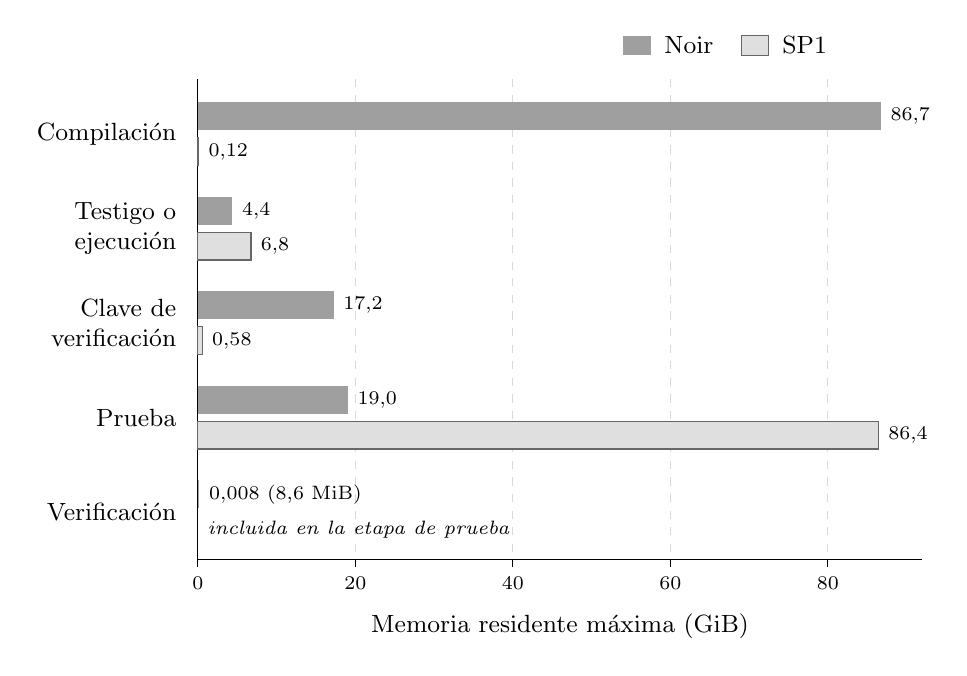
\begin{tikzpicture}[
		etapa/.style={anchor=east, font=\small, align=right},
		valor/.style={anchor=west, font=\scriptsize}
		]
		% Escala lineal: x = 0,1 cm por GiB
		\foreach \g in {0, 20, 40, 60, 80} {
			\draw[gray!30, dashed] (0.1*\g, 0.7) -- (0.1*\g, -5.4);
			\draw (0.1*\g, -5.4) -- (0.1*\g, -5.5) node[below, font=\scriptsize] {\g};
		}
		\draw (0, 0.7) -- (0, -5.4) -- (9.2, -5.4);
		\node[font=\small] at (4.6, -6.25) {Memoria residente máxima (GiB)};

		\foreach \y/\nombre/\ln/\vn/\ls/\vs in {
			0/Compilación/8.674/{86,7}/0.012/{0,12},
			-1.2/{Testigo o\\ejecución}/0.439/{4,4}/0.675/{6,8},
			-2.4/{Clave de\\verificación}/1.723/{17,2}/0.058/{0,58},
			-3.6/Prueba/1.905/{19,0}/8.645/{86,4}} {
			\node[etapa] at (-0.15, \y) {\nombre};
			\fill[gray!75] (0, \y+0.05) rectangle (\ln, \y+0.4);
			\node[valor] at (\ln, \y+0.225) {\vn};
			\fill[gray!25, draw=black!60] (0, \y-0.4) rectangle (\ls, \y-0.05);
			\node[valor] at (\ls, \y-0.225) {\vs};
		}
		\node[etapa] at (-0.15, -4.8) {Verificación};
		\fill[gray!75] (0, -4.75) rectangle (0.02, -4.4);
		\node[valor] at (0.02, -4.575) {0,008 (8,6 MiB)};
		\node[valor, font=\scriptsize\itshape] at (0, -5.025) {incluida en la etapa de prueba};

		% Leyenda
		\fill[gray!75] (5.4, 1.0) rectangle (5.75, 1.25);
		\node[valor, font=\small] at (5.8, 1.125) {Noir};
		\fill[gray!25, draw=black!60] (6.9, 1.0) rectangle (7.25, 1.25);
		\node[valor, font=\small] at (7.3, 1.125) {SP1};
	\end{tikzpicture}
	\caption[Memoria residente máxima por etapa en Noir y en SP1.]{Memoria residente máxima por
	etapa en Noir y en SP1. Ambas herramientas alcanzan un pico cercano a 86 GiB, Noir en la
	compilación y SP1 en cada generación de prueba.}
	\label{fig:resultados_memoria}
\end{figure}

\subsection{Costo en frío y amortización}
\label{sec:resultados_amortizacion}

La obtención de la primera prueba desde el código fuente demandó 92,3 minutos en Noir y
17,9 minutos en SP1, de modo que, para una única prueba, SP1 resulta unas cinco veces más rápido.
Esta comparación, sin embargo, no representa la operación del puente, en la que el mismo programa
genera una prueba por cada anclaje. La Tabla~\ref{tab:resultados_amortizacion} separa los costos
fijos de los costos por prueba según la Tabla~\ref{tab:metodologia_etapas}. El costo por prueba de
Noir, formado por el testigo y la prueba, asciende a 179,7 segundos, mientras que el de SP1, formado
por la etapa de prueba, asciende a 1029,5 segundos, es decir, unas 5,7 veces más. Si se considera
solo la generación de la prueba, la diferencia es de unas 12,2 veces.

\begin{table}[htbp]
	\centering
	\caption{Costos fijos, costos por prueba y tiempo total acumulado en Noir y en SP1.}
	\label{tab:resultados_amortizacion}
	\small
	\begin{tabular}{>{\raggedright\arraybackslash}p{6.2cm} >{\raggedleft\arraybackslash}p{3.2cm} >{\raggedleft\arraybackslash}p{3.2cm}}
		\toprule
		\textbf{Concepto} & \textbf{Noir} & \textbf{SP1} \\
		\midrule
		Costo fijo $t_{\mathrm{fijo}}$ & 5356,5 s (89,3 min) & 6,1 s (0,1 min) \\
		Costo por prueba $t_{\mathrm{prueba}}$ & 179,7 s (3,0 min) & 1029,5 s (17,2 min) \\
		\midrule
		$t_{\mathrm{total}}(1)$ & 92,3 min & 17,3 min \\
		$t_{\mathrm{total}}(7)$ & 110,2 min & 120,2 min \\
		$t_{\mathrm{total}}(20)$ & 149,2 min & 343,3 min \\
		$t_{\mathrm{total}}(50)$ & 239,0 min & 858,0 min \\
		\bottomrule
	\end{tabular}
\end{table}

Al sustituir estos valores en la Ecuación~\eqref{eq:punto_equilibrio} se obtiene
$n^{*} \approx 6{,}3$, de modo que, a partir de la séptima prueba generada con un mismo programa,
el tiempo total acumulado de Noir resulta inferior al de SP1. La
Figura~\ref{fig:resultados_equilibrio} representa ambas rectas. Este punto corresponde al circuito
de Noir medido en el servidor, por lo que el de los circuitos que integran el puente, que demuestran
el enunciado completo, puede diferir. El valor de
$t_{\mathrm{total}}(1)$ de SP1 es algo menor que su costo en frío porque este último incluye la
etapa de ejecución, que no forma parte del costo por prueba.

\begin{figure}[htbp]
	\centering
	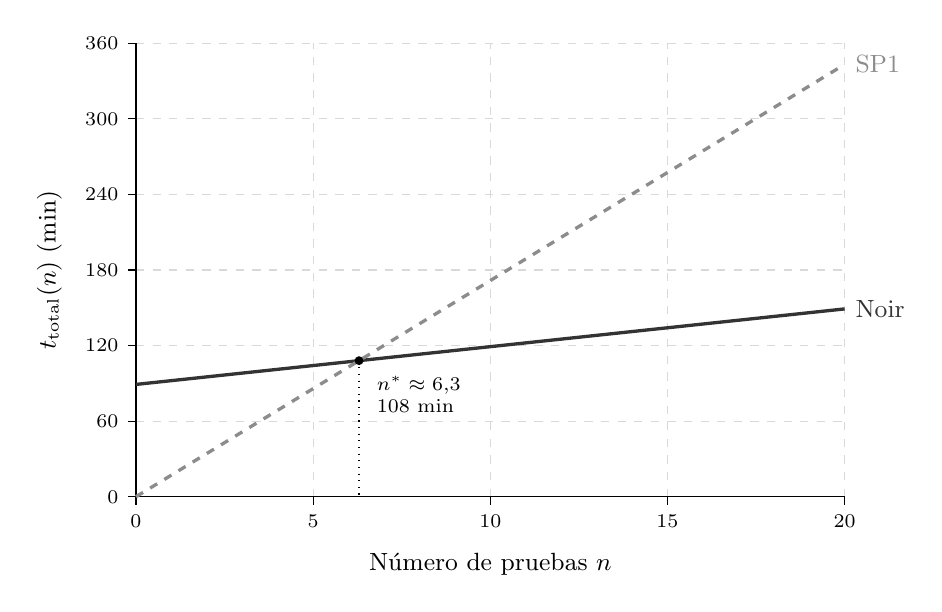
\begin{tikzpicture}[
		valor/.style={font=\scriptsize}
		]
		% Escalas: x = 0,45 cm por prueba; y = 0,016 cm por minuto
		\foreach \n in {0, 5, 10, 15, 20} {
			\draw[gray!30, dashed] (0.45*\n, 0) -- (0.45*\n, 5.76);
			\draw (0.45*\n, 0) -- (0.45*\n, -0.1) node[below, valor] {\n};
		}
		\foreach \m in {0, 60, 120, 180, 240, 300, 360} {
			\draw[gray!30, dashed] (0, 0.016*\m) -- (9, 0.016*\m);
			\draw (0, 0.016*\m) -- (-0.1, 0.016*\m) node[left, valor] {\m};
		}
		\draw (0, 5.76) -- (0, 0) -- (9, 0);
		\node[font=\small] at (4.5, -0.85) {Número de pruebas $n$};
		\node[font=\small, rotate=90] at (-1.1, 2.88) {$t_{\mathrm{total}}(n)$ (min)};

		\draw[very thick, black!80] (0, 1.428) -- (9, 2.387)
			node[right, font=\small] {Noir};
		\draw[very thick, black!45, dashed] (0, 0.002) -- (9, 5.492)
			node[right, font=\small] {SP1};

		\fill (2.833, 1.730) circle (1.6pt);
		\draw[dotted] (2.833, 1.730) -- (2.833, 0);
		\node[valor, anchor=north west, align=left, fill=white, inner sep=1.5pt] at (3.0, 1.6)
			{$n^{*} \approx 6{,}3$\\108 min};
	\end{tikzpicture}
	\caption[Tiempo total acumulado en función del número de pruebas.]{Tiempo total acumulado en
	función del número de pruebas generadas con un mismo programa, según la
	Ecuación~\eqref{eq:costo_total}. Las rectas se cortan en $n^{*} \approx 6{,}3$.}
	\label{fig:resultados_equilibrio}
\end{figure}

\subsection{Costo de verificación en la cadena de destino}
\label{sec:resultados_gas}

En la versión de Noir que integra el puente, el enunciado de consenso se verifica mediante dos
pruebas, puesto que el circuito completo no pudo compilarse en el equipo disponible
(Sección~\ref{sec:resultados_etapas}). El primer circuito, denominado en lo sucesivo circuito del
comité, comprueba que las claves recibidas corresponden al compromiso del comité registrado, que
participan al menos dos tercios de sus miembros, suma las claves de los participantes, deriva la
raíz de firma del encabezado y la transforma en un punto de $\mathbb{G}_2$, y vincula el hash del
bloque de ejecución con el encabezado y las raíces de transacciones y de recibos con ese bloque. El segundo, denominado
circuito de emparejamiento, verifica la Ecuación~\eqref{eq:bls_agregada}. Ambos exponen un mismo
valor público de enlace, calculado mediante la función de hash Poseidon2 sobre la clave agregada,
el punto del mensaje y la firma, y \texttt{BeaconLightClient} exige que ese valor coincida en las
dos pruebas, de modo que una prueba de emparejamiento de otra firma no puede combinarse con la
prueba del comité. Lo que conecta el consenso con la inclusión es el par formado por la raíz de
transacciones y la raíz de recibos, que el circuito del comité expone y que \texttt{BeaconLightClient}
registra de forma conjunta, mediante el hash Keccak de su concatenación. El contrato de acuñación
exige que ese par exacto esté registrado antes de aceptar la prueba de inclusión, de modo que no
es posible combinar la transacción de un bloque con el recibo de otro. La prueba de inclusión
demuestra, para una misma posición del mismo bloque, que la transacción figura en el árbol de
transacciones e invoca directamente \lstinline|lock| sobre \texttt{Sender}, que su recibo figura
en el árbol de recibos con una ejecución exitosa y que ese recibo contiene el evento
\texttt{Locked}, cuyos identificador, destinatario y monto deben coincidir con los de la
transacción.

La Tabla~\ref{tab:resultados_gas} reúne el gas de la verificación de cada prueba con las reglas
posteriores a Osaka y el tamaño de los datos que la acompañan, y la Figura~\ref{fig:resultados_gas}
compara el gas. Cada verificación de Noir requirió entre 4,49 y 4,75 millones de unidades de gas,
mientras que la verificación de una prueba Groth16 de SP1 requirió 259\,608 unidades según la
estimación, y la transacción correspondiente consumió 253\,395 según su recibo, ya que la
estimación puede superar el consumo efectivo. Cada verificación resulta, en consecuencia, entre
17,3 y 18,3 veces más costosa en Noir que en SP1, y las dos verificaciones que exige el enunciado
de consenso en Noir suman 9\,067\,892 unidades, unas 35 veces el costo de la verificación de SP1. El
código de los tres verificadores de Noir ocupa 17\,532, 17\,155 y 17\,407 bytes, por debajo del
límite de 24\,576 bytes que la propuesta EIP-170 impone al código de un contrato~\cite{eip170}.

\begin{table}[htbp]
	\centering
	\caption{Gas de ejecución de la verificación de cada prueba y tamaño de sus datos.}
	\label{tab:resultados_gas}
	\small
	\begin{tabular}{>{\raggedright\arraybackslash}p{3.9cm} >{\raggedright\arraybackslash}p{2.1cm} >{\raggedleft\arraybackslash}p{2.0cm} >{\raggedleft\arraybackslash}p{1.9cm} >{\raggedleft\arraybackslash}p{3.0cm}}
		\toprule
		\textbf{Prueba} & \textbf{Sistema} & \textbf{Gas} & \textbf{Prueba (bytes)} &
		\textbf{Entradas públicas} \\
		\midrule
		Comité en Noir ($2^{22}$ filas) & UltraHonk & 4\,489\,878 & 11\,072 & 7 elementos \\
		\addlinespace
		Emparejamiento en Noir ($2^{23}$ filas) & UltraHonk & 4\,578\,014 & 11\,456 & 1 elemento \\
		\addlinespace
		Inclusión en Noir ($2^{22}$ filas) & UltraHonk & 4\,745\,084 & 11\,072 & 168 elementos \\
		\addlinespace
		Prueba de SP1 & Groth16 & 259\,608 & 356 & 577 bytes \\
		\bottomrule
	\end{tabular}

	\vspace{0.5em}
	\begin{minipage}{0.95\textwidth}
		\footnotesize
		El gas corresponde a las reglas posteriores a Osaka e incluye el costo intrínseco y el de los
		datos de la transacción. La cifra de SP1 corresponde a \texttt{eth\_estimateGas} con las
		reglas de Cancun, válidas también después de Osaka para este verificador
		(Sección~\ref{sec:metodologia_gas}). La prueba de SP1 pertenece a otro programa, y los
		valores públicos del programa de consenso ocupan 320 bytes.
	\end{minipage}
\end{table}

\begin{figure}[htbp]
	\centering
	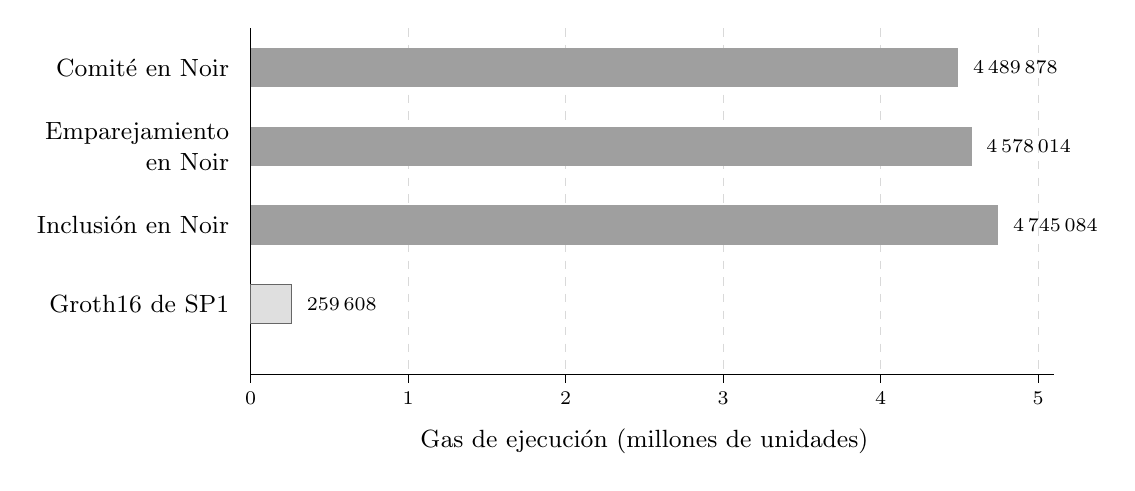
\begin{tikzpicture}[
		etapa/.style={anchor=east, font=\small, align=right},
		valor/.style={anchor=west, font=\scriptsize}
		]
		% Escala lineal: x = 2 cm por millón de unidades de gas
		\foreach \m in {0, 1, 2, 3, 4, 5} {
			\draw[gray!30, dashed] (2*\m, 0.5) -- (2*\m, -3.9);
			\draw (2*\m, -3.9) -- (2*\m, -4.0) node[below, font=\scriptsize] {\m};
		}
		\draw (0, 0.5) -- (0, -3.9) -- (10.2, -3.9);
		\node[font=\small] at (5, -4.75) {Gas de ejecución (millones de unidades)};

		\fill[gray!75] (0, -0.25) rectangle (8.980, 0.25);
		\node[etapa] at (-0.15, 0) {Comité en Noir};
		\node[valor] at (9.05, 0) {4\,489\,878};

		\fill[gray!75] (0, -1.25) rectangle (9.156, -0.75);
		\node[etapa] at (-0.15, -1) {Emparejamiento\\en Noir};
		\node[valor] at (9.22, -1) {4\,578\,014};

		\fill[gray!75] (0, -2.25) rectangle (9.490, -1.75);
		\node[etapa] at (-0.15, -2) {Inclusión en Noir};
		\node[valor] at (9.56, -2) {4\,745\,084};

		\filldraw[fill=gray!25, draw=black!60] (0, -3.25) rectangle (0.519, -2.75);
		\node[etapa] at (-0.15, -3) {Groth16 de SP1};
		\node[valor] at (0.59, -3) {259\,608};
	\end{tikzpicture}
	\caption[Gas de ejecución de la verificación de cada prueba.]{Gas de ejecución de la
	verificación de cada prueba en la cadena de destino con las reglas posteriores a Osaka, según la
	Tabla~\ref{tab:resultados_gas}.}
	\label{fig:resultados_gas}
\end{figure}

La Tabla~\ref{tab:resultados_gas_tx} recoge el gas de las transacciones completas de Noir con
ambas versiones de las reglas. La transacción de anclaje, que verifica las dos pruebas de consenso y
registra el par de raíces del bloque, consumió 9\,082\,703 unidades, y la de acuñación, que verifica la
prueba de inclusión, aplica los controles de las entradas públicas y del identificador del bloqueo
y acuña el activo, 4\,873\,158. El anclaje se paga una vez por bloque anclado y lo comparten todas
las transferencias incluidas en ese bloque, mientras que la acuñación se paga en cada
transferencia. La verificación de las pruebas representa prácticamente la totalidad de ambos
costos. La diferencia entre el gas del anclaje y la suma de sus dos verificaciones es de solo
14\,811 unidades, y la verificación de inclusión equivale al 97,4\,\% del gas de la acuñación, cuya
diferencia, de 128\,074 unidades, aproxima el costo de los controles y de la acuñación. El anclaje
utiliza el 54,1\,\% del límite de 16\,777\,216 unidades por transacción que establece la propuesta
EIP-7825~\cite{eip7825}, de modo que el diseño en dos pruebas cabe en una sola transacción. La comprobación del árbol de
transacciones, que se incorporó a la prueba de inclusión después de la del árbol de recibos,
incrementó el gas de la acuñación en 59\,465 unidades, desde 4\,813\,693, principalmente por las
32 entradas públicas que añade la raíz de transacciones.

\begin{table}[htbp]
	\centering
	\caption{Gas de las transacciones de Noir según la versión de las reglas de la EVM.}
	\label{tab:resultados_gas_tx}
	\small
	\begin{tabular}{>{\raggedright\arraybackslash}p{6.4cm} >{\raggedleft\arraybackslash}p{2.6cm} >{\raggedleft\arraybackslash}p{2.6cm} >{\raggedleft\arraybackslash}p{1.8cm}}
		\toprule
		\textbf{Operación} & \textbf{Osaka} & \textbf{Prague} & \textbf{Aumento} \\
		\midrule
		Anclaje (\texttt{update}), con dos verificaciones & 9\,082\,703 & 6\,215\,537 & 46,1\,\% \\
		\addlinespace
		Verificación de la prueba del comité & 4\,489\,878 & 3\,077\,258 & 45,9\,\% \\
		\addlinespace
		Verificación de la prueba de emparejamiento & 4\,578\,014 & 3\,133\,115 & 46,1\,\% \\
		\addlinespace
		Acuñación (\texttt{release}), con una verificación & 4\,873\,158 & 3\,455\,948 & 41,0\,\% \\
		\addlinespace
		Verificación de la prueba de inclusión & 4\,745\,084 & 3\,332\,963 & 42,4\,\% \\
		\bottomrule
	\end{tabular}

	\vspace{0.5em}
	\begin{minipage}{0.95\textwidth}
		\footnotesize
		La columna Osaka corresponde a Anvil con la bifurcación BPO1 y la columna Prague a la red de
		Hardhat.
	\end{minipage}
\end{table}

Las reglas de Osaka elevaron el gas de las transacciones de Noir entre un 41,0 y un 46,1\,\%
respecto de las de Prague, como consecuencia del incremento del costo del precompilado MODEXP que
introdujo la propuesta EIP-7883~\cite{eip7883} y que el verificador de UltraHonk emplea. El
verificador de SP1 no emplea ese precompilado (Sección~\ref{sec:metodologia_gas}), por lo que su
costo no varió. La ventaja de SP1 en la verificación aumentó, en consecuencia, con la actualización.
Con las reglas de Prague, la verificación de la prueba de inclusión de Noir costaba unas 12,8 veces
la de SP1, y con las posteriores a Osaka, unas 18,3 veces.

La diferencia procede de los sistemas de prueba que verifica cada contrato. El verificador Groth16
realiza una cantidad fija de operaciones sobre la curva BN254, independiente del tamaño del
programa (Sección~\ref{sec:snarks_starks}), y su componente principal es una comprobación de
emparejamiento de cuatro pares. En Optimism Sepolia, ese emparejamiento cuesta 181\,000 unidades
de gas, valor que coincide con el de la propuesta EIP-1108, de 45\,000 unidades más 34\,000 por
par~\cite{eip1108}, y que equivale a cerca del 70\,\% de la verificación medida. En la misma red se
comprobaron también los precios de la suma y de la multiplicación escalar sobre la curva, de 150 y
6\,000 unidades, respectivamente. El verificador de UltraHonk, en cambio, recalcula los desafíos de
Fiat-Shamir, verifica el protocolo \textit{sumcheck}, cuyo número de rondas crece con el logaritmo
del tamaño del circuito, y procesa cada entrada pública (Sección~\ref{sec:noir_impl_publicas}). Los
circuitos del comité y de inclusión tienen el mismo tamaño, de $2^{22}$ filas, y pruebas de igual
longitud, de modo que la diferencia de 255\,206 unidades entre sus verificaciones se atribuye a las
161 entradas públicas adicionales del segundo, a razón de unas 1\,585 unidades por entrada,
incluido el costo de sus 32 bytes de datos. El circuito de emparejamiento duplica el tamaño del
circuito del comité con seis entradas menos, y su verificación cuesta 88\,136 unidades más, lo que
equivale a unas 98\,000 unidades por duplicación del tamaño, incluidos los 384 bytes adicionales
de su prueba. Las entradas públicas del circuito de inclusión cuestan, por lo tanto, más que dos
duplicaciones del tamaño del circuito. En Noir, el costo de verificación depende en gran medida
del número de entradas públicas, lo que confirma la relevancia de la descomposición de los valores
públicos señalada en la Sección~\ref{sec:noir_impl_publicas}. El circuito del comité, que
representa cada una de las dos raíces en dos mitades de 128 bits, expone solo siete entradas, mientras que
el de inclusión representa cada byte en un elemento.

En SP1, el costo de la verificación no depende del programa probado, salvo a través de los valores
públicos. La prueba empleada en la medición acompaña valores públicos de 577 bytes, frente a los
320 del programa de consenso. El cálculo aislado del hash de cada secuencia, ejecutado como una
transacción completa, requirió 29\,072 y 25\,825 unidades de gas, respectivamente, y 1\,384 y
1\,221 unidades una vez descontados el costo intrínseco y el de los datos de la transacción. La
diferencia atribuible a los valores públicos es, en consecuencia, de 3\,247 unidades, equivalente
al 1,3\,\% de la verificación medida, por lo que el valor de la Tabla~\ref{tab:resultados_gas}
representa con una aproximación suficiente el costo de verificar una prueba del programa de
consenso.

La lógica de \texttt{BeaconLightClient} de SP1, medida con el verificador simulado, requirió
84\,036 unidades de gas en el primer anclaje y 66\,936 en los anclajes siguientes. La diferencia,
de 17\,100 unidades, corresponde a la escritura del último \textit{slot} registrado, que cuesta
22\,100 unidades cuando se realiza por primera vez y 5\,000 cuando actualiza un valor existente.
El registro del hash del bloque anclado exige en ambos casos una escritura nueva, de 22\,100
unidades. La rotación del compromiso del comité, que el propietario realiza mediante una
transacción separada (Sección~\ref{sec:puente_aceptacion}), requirió 30\,127 unidades. Si al gas
del verificador se suma el de la lógica del contrato y se descuenta una vez el costo intrínseco de
la transacción, se obtienen unas 305\,544 unidades para un anclaje ordinario y 322\,644 para el
primero. Estas cifras son sumas de componentes medidos y no la medición de una transacción
completa, puesto que conservan el costo de los datos de ambas llamadas y el de la llamada al
verificador simulado. Con esa salvedad, el anclaje de Noir consume unas 30 veces el gas estimado
para el anclaje de SP1. La verificación de la prueba de inclusión de SP1 no se midió. Como su
verificador es el mismo y sus valores públicos ocupan quince palabras de 32 bytes, es decir,
480 bytes, cabe esperar un costo del mismo orden que el de la Tabla~\ref{tab:resultados_gas},
aunque esta estimación no sustituye a una medición.

El tamaño de los datos incide, además, en la tarifa de datos de la capa 1 de Optimism
(Sección~\ref{sec:op_tarifas}). Las dos pruebas de consenso de Noir y sus ocho entradas públicas
ocupan 22\,784 bytes, y la prueba de inclusión con sus 168 entradas, 16\,448 bytes, mientras que la
llamada completa al verificador de SP1 ocupó 1\,156 bytes, que incluyen la prueba de 356 bytes y
los valores públicos de 577 bytes. Los datos de un anclaje y de una acuñación de Noir son, por lo
tanto, unas 20 y 14 veces mayores, respectivamente, que los de una verificación de SP1, y esa
diferencia se traslada a la tarifa de datos de la capa 1, que depende del tamaño comprimido de la
transacción~\cite{opfees}. A la ejecución en la capa 2 y a la tarifa de datos se suma, desde la
actualización Isthmus, una tarifa del operador~\cite{opfees}, de modo que el costo monetario de una
transacción solo puede establecerse enviándola a la red. Ese costo no se midió en este trabajo.

El flujo completo del puente de Noir se ejecutó, por último, de punta a punta. Con la versión final de
todos los circuitos, se bloquearon 42 GUA en Ethereum Sepolia, mediante una transacción de
tipo EIP-1559 en la posición 97 del bloque 12\,122\,052, y la prueba de consenso se generó a
partir de la firma del comité en el \textit{slot} 11\,565\,990, con la participación de 509 de sus 512
miembros. La cadena de destino fue una red local de Anvil con las reglas posteriores a Osaka, en la
que el propietario registró el compromiso del comité del período 1411 mediante
\lstinline|setCommittee|. Ambas transacciones fueron aceptadas y el destinatario recibió los
42 GUA. Las 33 pruebas automatizadas de los contratos y las 30 del circuito de inclusión
concluyeron con éxito, incluidas las de rechazo descritas en la Sección~\ref{sec:metodologia_gas}.
En el circuito del comité, con datos reales, se comprobó además el rechazo de una participación
inferior a dos tercios, de una clave ajena al comité y de raíces de transacciones o de recibos
falsas.

\subsection{Discusión}
\label{sec:resultados_discusion}

En la operación del puente, el programa de consenso se mantiene fijo mientras no se modifique su
código, puesto que el comité, la firma y el encabezado son entradas y no parte del circuito. La
rotación del comité, que ocurre aproximadamente cada 27 horas, no exige por lo tanto recompilar el
programa ni regenerar su clave de verificación. En consecuencia, el costo fijo de Noir se paga una
vez por versión del programa y el punto de equilibrio se supera con las primeras siete pruebas. A
partir de ese punto, cada anclaje cuesta unos 3 minutos de generación en Noir frente a unos
17 minutos en SP1. La frecuencia de anclaje determina cuán rápido se alcanza ese punto, pero no lo
modifica.

La memoria constituye una diferencia práctica de igual importancia. Ambas herramientas alcanzan un
pico de unos 86 GiB, pero en momentos distintos. En Noir, ese pico corresponde a la compilación,
que puede realizarse una sola vez y en un equipo distinto del que opera el \textit{relayer},
puesto que el circuito compilado y la clave de verificación se conservan como archivos. El equipo
que genera las pruebas necesita entonces unos 19 GiB de memoria en el circuito medido, y los
circuitos que integran el puente se probaron en un equipo de 18 GB, aunque la memoria máxima de
esa generación no se midió. En SP1, el pico corresponde a
cada generación de prueba, de modo que el equipo del \textit{relayer} debe disponer en todo momento
de una memoria del orden de 90 GiB. Este requisito incide directamente en el costo de la máquina en
la nube que opera el puente.

La situación se invierte durante el desarrollo. Cada modificación del circuito de Noir exige
repetir la compilación, de casi una hora y media, y la obtención de la clave de verificación,
mientras que en SP1 la recompilación del programa invitado no impone una etapa equivalente de
obtención de la clave, que se deriva en segundos del ejecutable, aunque la duración de la
compilación misma no se midió (Sección~\ref{sec:metodologia_validez}). SP1 permite,
además, ejecutar el programa sin generar la prueba y obtener el número de ciclos en pocos segundos,
lo que facilita depurar el programa y estimar su costo antes de probarlo. Esta diferencia favorece a
SP1 en la flexibilidad de desarrollo, una de las dos dimensiones de la pregunta de investigación.

Los resultados deben interpretarse a la luz de las condiciones de la
Sección~\ref{sec:metodologia_validez}, varias de las cuales afectan de forma desigual a ambas
herramientas. La medición de SP1 corresponde a un caso desfavorable, ya que la prueba se generó solo
en el procesador y el programa no emplea los precompilados de SHA-256 ni de BLS12-381, de modo que
la aritmética de la curva, que domina los 66,4 millones de ciclos, se ejecuta como instrucciones
ordinarias (Sección~\ref{sec:sp1_limitaciones}). El uso de precompilados, de aceleración por GPU o
de la red de probadores~\cite{succinctnetwork} reduciría previsiblemente el costo por prueba de SP1,
y con él el punto de equilibrio, aunque esa reducción no se cuantificó en este trabajo. En sentido
contrario, la prueba de SP1 medida es la prueba de núcleo, cuyo tamaño crece con la ejecución y que
el contrato de destino no puede verificar. Obtener la prueba Groth16 que exige el puente añade la
compresión recursiva y la envoltura (Sección~\ref{sec:sp1_impl_integracion}), cuyo tiempo no se
incluye en las mediciones y aumentaría el costo por prueba de SP1. La prueba UltraHonk de Noir, en
cambio, tiene un tamaño fijo para cada circuito, que crece con el logaritmo de su tamaño y es de
11\,072 bytes para los circuitos de $2^{22}$ filas y de 11\,456 bytes para el de $2^{23}$
(Sección~\ref{sec:resultados_gas}), y su verificación local demandó 0,01 segundos. El circuito de
Noir medido en el servidor demuestra, por otra parte, un enunciado menor que el de SP1, lo que
favorece a Noir en la comparación de los tiempos de generación. En el computador de 18 GB, sin
embargo, los dos circuitos que demuestran el enunciado completo se probaron en unos 98 segundos,
un valor del mismo orden que el costo por prueba de Noir en el servidor, lo que sugiere, sin
constituir una medición comparable, que su ventaja en el costo por prueba no se debe a la
reducción del enunciado. Su variante compatible con
la EVM difiere de la medida, a lo sumo, en la función de hash empleada para derivar los
desafíos del protocolo, por lo que no se espera que modifique el orden de magnitud de los
resultados, aunque esa diferencia no se midió.

El costo de verificación en la cadena de destino invierte la ventaja observada en la generación.
Con las reglas vigentes en la cadena de destino, la verificación de una prueba Groth16 de SP1
requiere entre 17 y 18 veces menos gas que cada prueba UltraHonk de Noir y unas 35 veces menos que
las dos pruebas que exige el enunciado de consenso en Noir, y sus datos ocupan entre 14 y 20 veces
menos, lo que reduce también la tarifa de datos de la capa 1. Esta ventaja se obtiene, sin embargo, a cambio de la envoltura
Groth16, cuyo tiempo de generación no se midió, de modo que la comparación completa enfrenta un
mayor costo de generación por prueba en SP1 con un menor costo de verificación por transacción. El
costo de verificación se paga en cada anclaje y en cada acuñación, y lo paga quien presenta las
pruebas, mientras que el de generación lo soporta el equipo del probador. La elección entre ambas
herramientas depende, en consecuencia, de cuál de esos dos costos resulte determinante para la
operación del puente.

En relación con la pregunta de investigación, los resultados indican que, para la verificación de
la firma agregada del comité de sincronización, SP1 ofrece una ventaja clara en la flexibilidad de
desarrollo, en el costo de la primera prueba y en el costo de verificación en la cadena de destino,
pero no en el tiempo de generación de las pruebas en operación, en el que Noir resulta unas 5,7
veces más rápido por prueba y requiere unas cuatro veces menos memoria. Las mediciones de
generación se limitan al programa de consenso, al procesador como único recurso de cómputo y a una
sola ejecución por etapa, y en Noir corresponden a un circuito que demuestra un enunciado menor que
el de SP1. Las de verificación excluyen las transacciones completas de anclaje y de acuñación de
SP1, la verificación de su prueba de inclusión y el costo monetario de las transacciones. El
Capítulo~\ref{chp:conclusion} retoma estos resultados para responder la pregunta de investigación
y verificar la hipótesis.
